As stated in the previous chapter, one of the main limitations displayed by the
Hodgkin-Huxley model is the fact that it can produce only a small fraction of the
activity patterns commonly observed in experiments. Said so, it would be desirable to
build a model able to reproducing virtually all the possible patterns of activity.
\begin{figure}[H]
    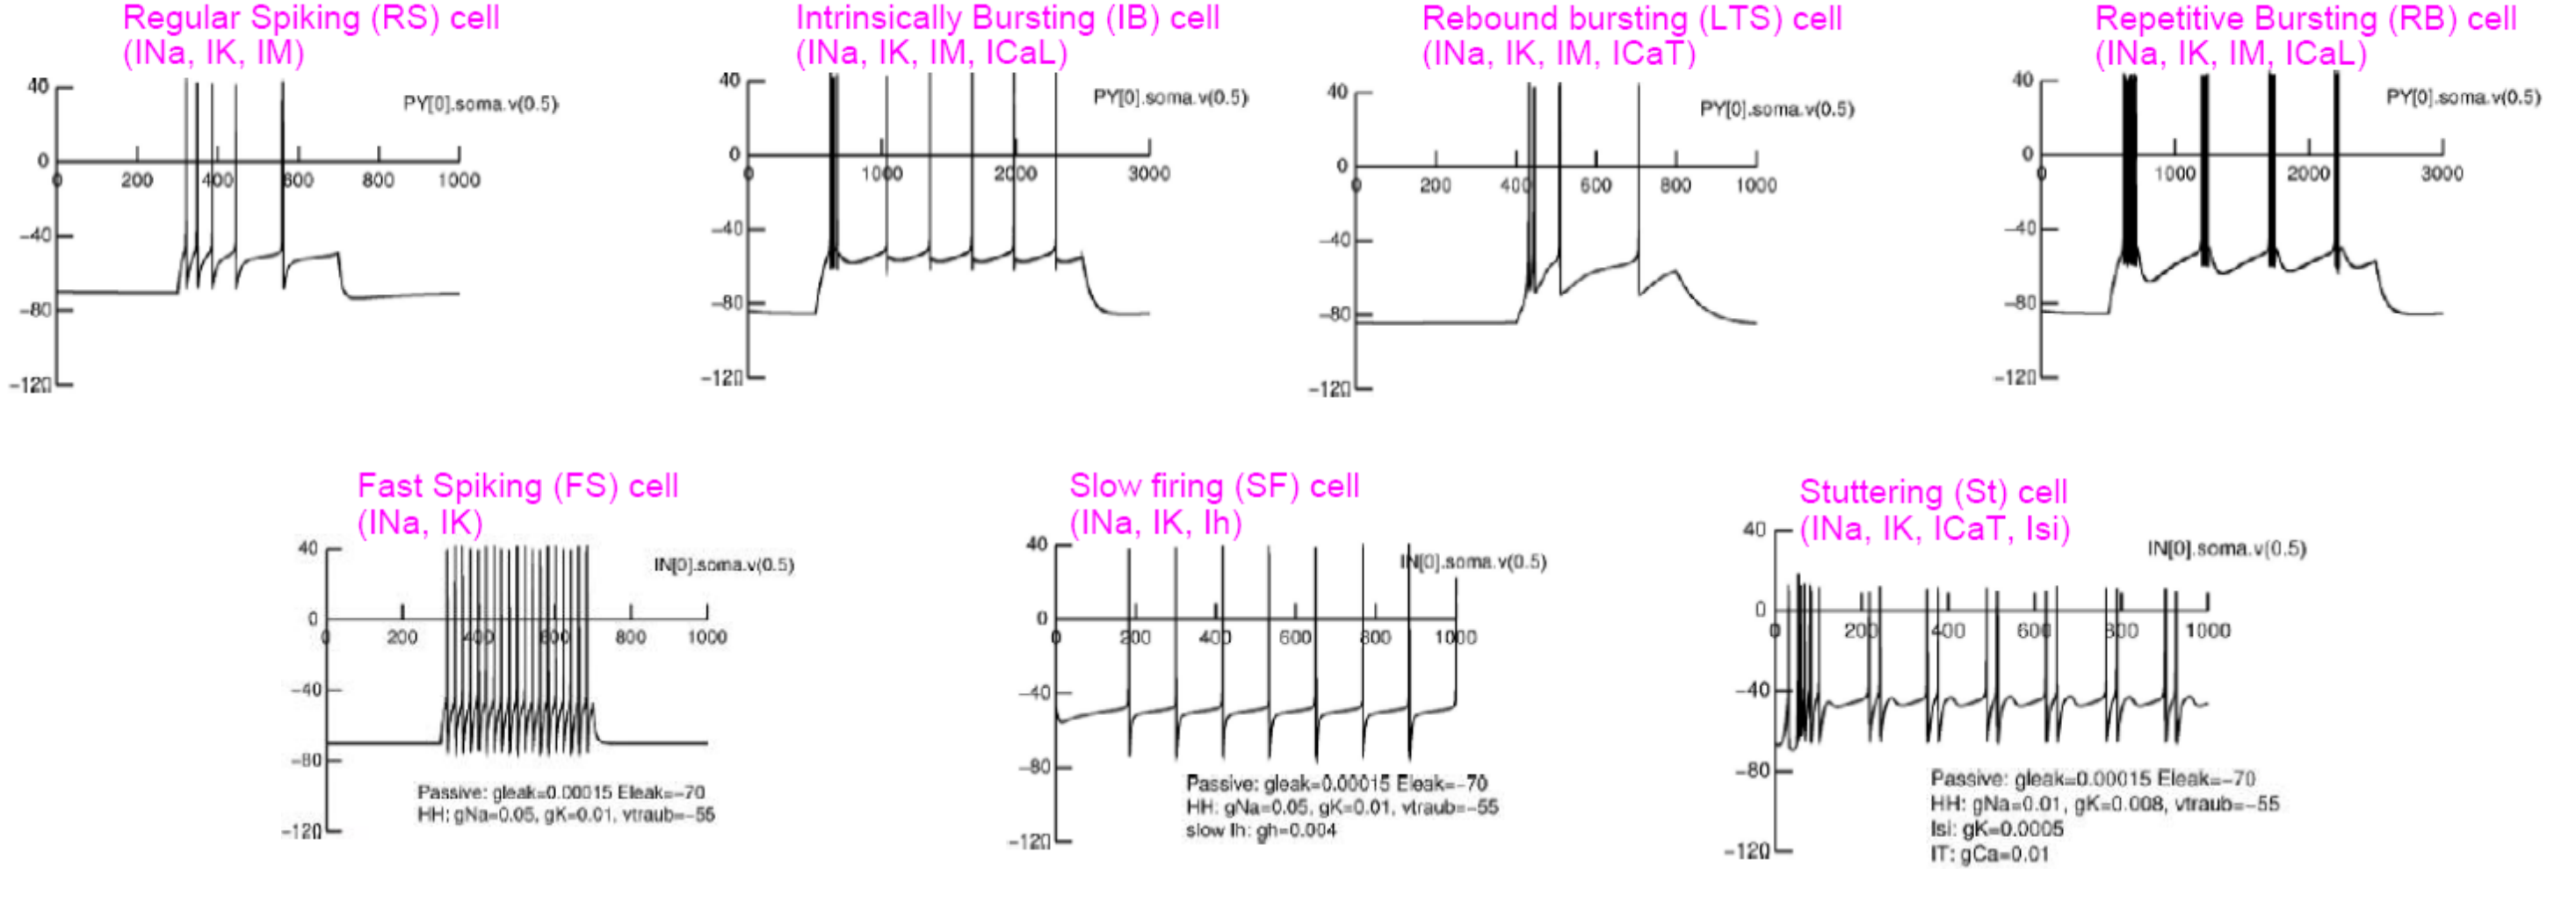
\includegraphics[scale=0.26]{06_1}
    \centering
\end{figure}
Note that these different patterns are a consequence of different ionic channels being
involved, each one with a different kinetics.
\begin{itemize}
    \item \textbf{Inward currents}: sodium current (fast), sodium current (persistent),
          calcium current (low-threshold), calcium current (high-threshold).
    \item \textbf{Outward currents}: potassium current (several families of channels).
\end{itemize}
A generic ionic current for the ions of type \(j\) can be formalized as follow:
\begin{equation*}
    I_{j}=\bar{g}_{j}\cdot{m^{p_{j}}h^{q_{j}}}\cdot{(V_{m}-E_{j})}
\end{equation*}
where the \(m\) gating particle is activating and \(h\) inactivating.

\subsection{Channels Types}
\subsubsection{Sodium Channels}
\paragraph{Fast Sodium Channels (\(I_{Na}\))} This is the kind of sodium chnnels
considered in the HH model, described by
\begin{equation*}
    I_{Na}=\bar{g}_{Na}\cdot{m^{3}h}\cdot{(V_{m}-E_{Na})}
\end{equation*}
\paragraph{Persistent Sodium Channels (\(I_{NaP}\))} This type of channel has \(q_{NaP}=0\),
therefore it is described by
\begin{equation*}
    I_{NaP}=\bar{g}_{NaP}\cdot{m}\cdot{(V_{m}-E_{Na})}
\end{equation*}
Note that if a neuron with only persistent sodium channels is considered, it would
constantly depolarize.\\
In addition to this consideration, the time constants of sodium gating particles are
comparable, thus sodium channels are responsible for hyperpolarization and depolarization,
but they are not able to produce spikes on their own.
\subsubsection{Potassium Channels}
\paragraph{Rapidly Inactivating Potassium Channels (\(I_{A}\))} They present two distinct
subtypes and have a time constant \(\tau_{h}\approx{10\;ms}\).
\paragraph{Slowly Inactivating Potassium Channels (\(I_{K}\))} They present two distinct
subtypes and have a time constant \(\tau_{h}\approx{200\;ms}\).\\
Note that the time constant of potassium \(\tau_{h,A}>>\tau_{h,Na}\), therefore the ionic
current \(I_{A}\) tends to hyperpolarize the membrane potential, slowing down the firing
rate: new action potentials occur as soon as the \(I_{A}\) current has become sufficiently
inactivated. Hence, the HH model in conjunction with these families of potassium channels
is able to model \textbf{Type I} neurons, even with very low firing frequencies, as
visible in the plot below.
\begin{figure}[H]
    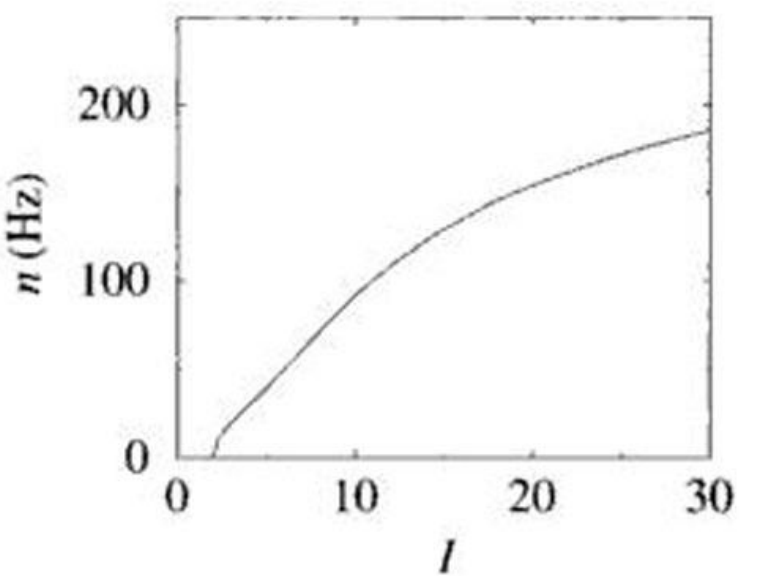
\includegraphics[scale=0.35]{06_2}
    \centering
\end{figure}
\subsubsection{Calcium Channels}
Differently from Na\({}^{+}\) and K\({}^{+}\), the concentration of Ca\({}^{2+}\) ions
is extremely low inside a cell and it is significantly affected by the calcium influx
occuring during an action potential. In particular, calcium has two functions in the
generation of an action potential:
\begin{itemize}
    \item Carry a positive electrical charge, contributing to depolarization.
    \item Modulate the activity of other channels, being a second messenger.
\end{itemize}
\paragraph{Low-Threshold Calcium Channels (\(I_{T}\))} These are inactivating channels,
similar to \(I_{Na}\), but differring in the shifting of the activation and inactivation
curves towards a hyperpolarized membrane potential: these channels are completely
inactivated at resting potential. In this case, an action potential can be elicited
by an inhibitory (hyperpolarizing) input, as a matter of fact, when it is switched off,
an overshoot of the action potential is observed, due to a quick depolarization of the
membrane, generating a low-threshold calcium spike: this phenomenon is known as
post-inhibitory rebound.
\begin{figure}[H]
    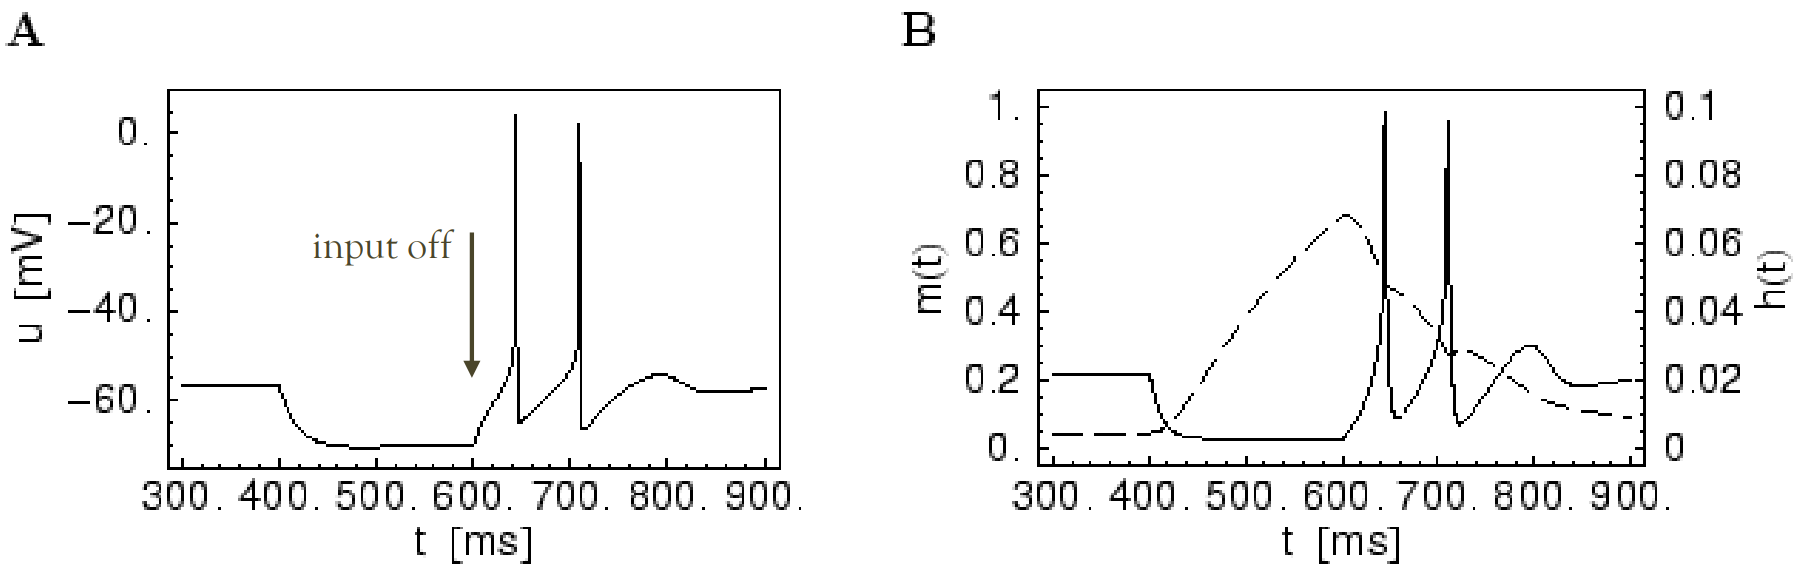
\includegraphics[scale=0.28]{06_3}
    \centering
\end{figure}
\paragraph{High-Threshold Calcium Channels (\(I_{L}\))} These channels produce a
non-inactivating current, which can be activated only at high levels of depolarization.
For instance, this current is responsible for the generation of bursting patterns.
\begin{equation*}
    I_{L}=\bar{g}_{Ca}\cdot{m^{2}}\cdot{(V_{m}-E_{Ca})}
\end{equation*}
\subsubsection{Calcium-Activated Potassium Channels}
There are two main families of calcium-activated potassium channels:
\begin{itemize}
    \item \textbf{\(I_{C}\)}: these channels depends on both voltage and Ca\({}^{2+}\)
          concentration.
          \begin{equation*}
              I_{C}=\bar{g}_{C}\cdot{m}\cdot{(V_{m}-E_{K})}
          \end{equation*}
    \item \textbf{\(I_{AHP}\)}: these channels are slower than the \(I_{C}\) ones and they
          depend solely on Ca\({}^{2+}\) concentration.
          \begin{equation*}
              I_{AHP}=\bar{g}_{AHP}\cdot{m}\cdot{(V-E_{K})}
          \end{equation*}
          Note that \(I_{AHP}\) is a non-inactivating current and due to the low time constant,
          each spike increases the activation of the gating particle \(m\). If the neuron is
          stimulated by a constant depolarizing current, each action potential elicited increases
          the amount of open AHP channels, therefore the corresponding  \(I_{K}\) is
          subtracted from the applied stimulus. This causes a decrease in the firing frequency:
          such a phenomenon is called adaptation.
          \begin{figure}[H]
              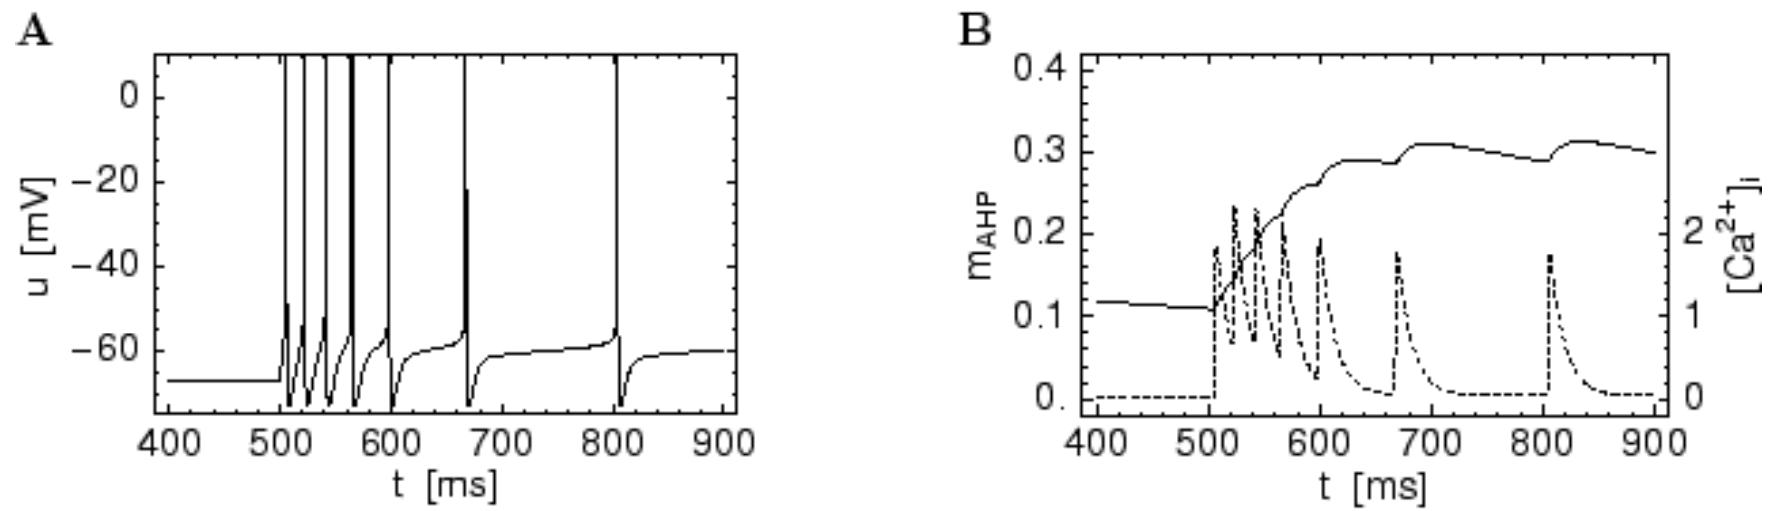
\includegraphics[scale=0.28]{06_4}
              \centering
          \end{figure}
\end{itemize}
Finally, the differential equation describing the model of a neuron (compartment \(k\))
can be as:
\begin{equation*}
    C_{k}\frac{dV_{k}}{dt}=\sum_{j}g_{j,k}(V_{j}-E_{k})-I_{ionic,k}
\end{equation*}
The ionic channels to consider are distributed as follow:
\begin{itemize}
    \item Na\({}^{+}\) channels: 2
    \item Leakage channels: 1
    \item K\({}^{+}\) channels: 6
    \item Ca\({}^{2+}\) channels: 2
\end{itemize}

\subsection{Stimulation and Activity Patterns}
Note that when stimulating a neuron it is important to carefully select the stimulation
amplitude and the location where it is delivered, as they both affect the neuron response.
\begin{figure}[H]
    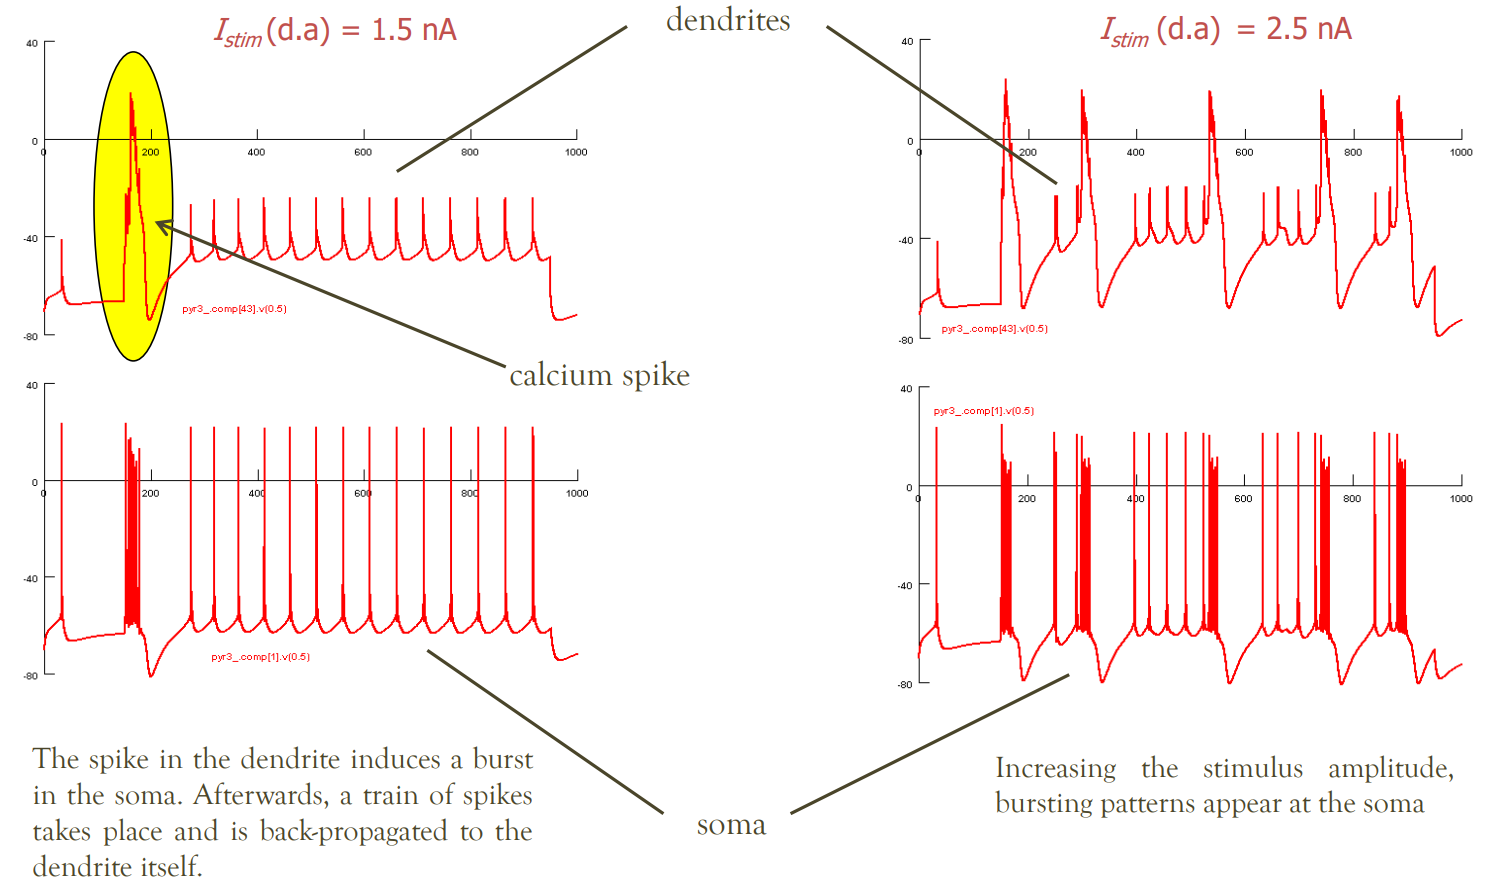
\includegraphics[scale=0.4]{06_5}
    \centering
\end{figure}
Apart from typical spikes, other kinds of activation might be observed:
\begin{itemize}
    \item \textbf{Spikelets}: small action potentials with an amplitude below \(10\;mV\).
    \item \textbf{Partial Spikes}: action potentials with an amplitude ranging from \(10\)
          to \(25\;mV\).
\end{itemize}
\begin{figure}[H]
    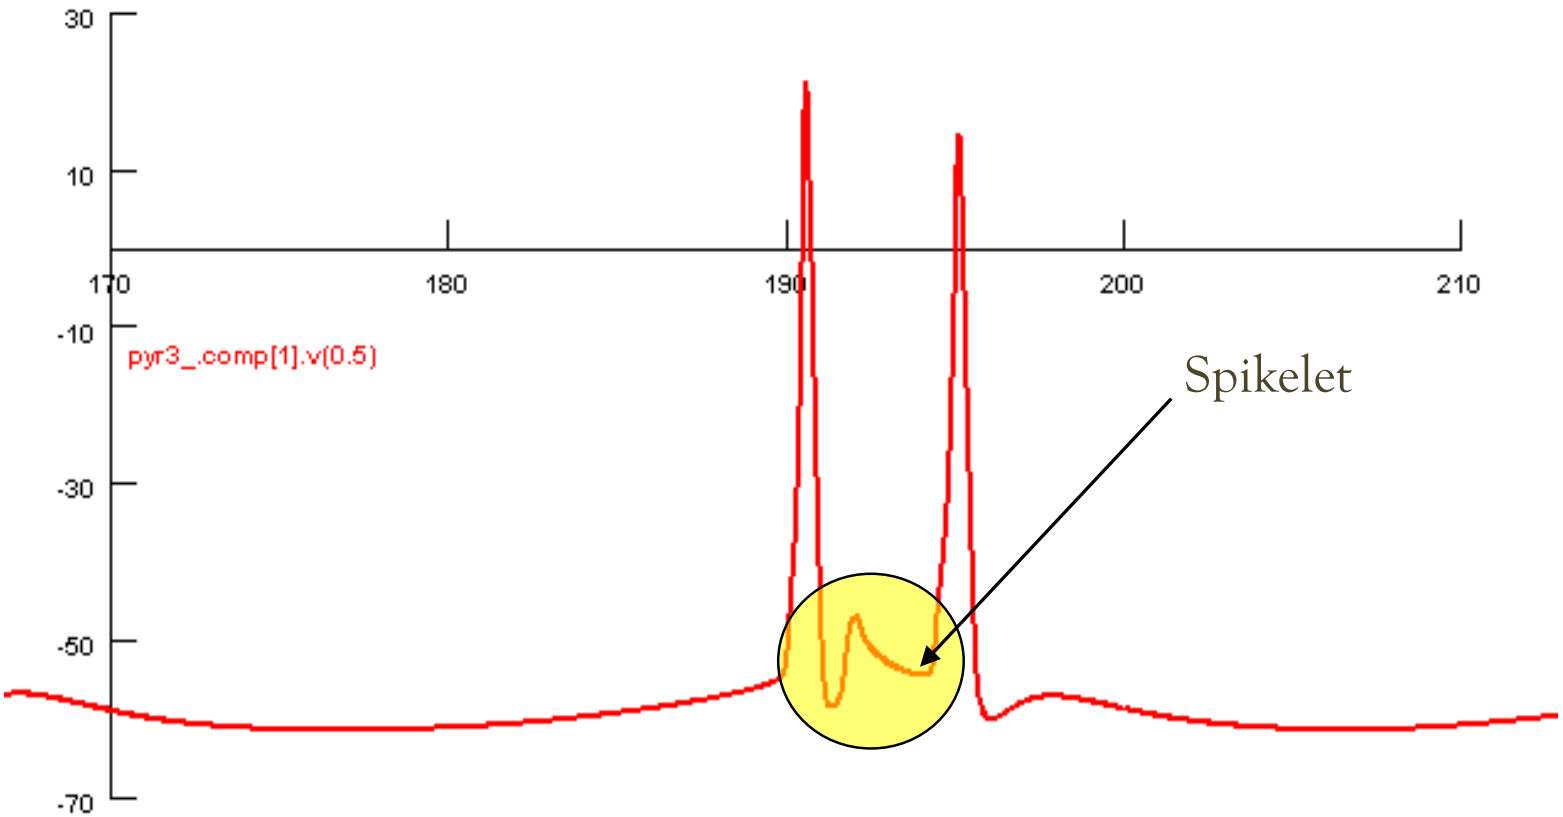
\includegraphics[scale=0.24]{06_6}
    \centering
\end{figure}
Also bursts are not all identical, but they might present different features according to
the stimulation site.
\paragraph{Apical Dendrites} A stimulation there may evoke both small spikes (due to fast
Na\({}^{+}\) channels) and spike trains separated by action potentials due to the
slow high-threshold Ca\({}^{2+}\) channels kinetics.
\paragraph{Soma} In the soma there are no calcium channels, as they exist only in the
dendrites. A more rythmic activity is thus induced, in addition the stimulation amplitude
highly shapes the response. Note that persistent Na\({}^{+}\) channels play a crucial role
in switching from rythmic spiking to rythmic bursting in the soma.